\documentclass[a4paper,14pt]{report}
\usepackage[utf8]{inputenc}
\usepackage[ukrainian]{babel}
\usepackage{amsmath,amsfonts,amssymb}
\usepackage{graphicx}
\usepackage{geometry}
\usepackage{fancyhdr}
\usepackage{titlesec}
\usepackage{indentfirst}
\usepackage{caption}
\usepackage{listings}
\usepackage{hyperref}
\usepackage{float}
\usepackage{tocloft}
\usepackage{enumitem}
\usepackage{pdfpages} % для вставки титульного аркуша, якщо він як PDF

\graphicspath{ {./img/} }


\geometry{left=3cm, right=1.5cm, top=2cm, bottom=2cm}
\setlength{\parindent}{1.25cm}
\setlength{\parskip}{0.5em}

% Стилі заголовків
\titleformat{\section}{\Large\bfseries\centering}{РОЗДІЛ \thesection.}{1em}{\MakeUppercase}
\titleformat{\subsection}{\normalsize\bfseries}{\thesubsection.}{0.5em}{}

% Стиль для змісту
\renewcommand{\cftsecleader}{\cftdotfill{\cftdotsep}}
\usepackage{titlesec}
\titleformat{\section}[block]{\center\normalfont\Large\bfseries}{\thesection}{1em}{}

\def\changemargin#1#2{\list{}{\rightmargin#2\leftmargin#1}\item[]}
\let\endchangemargin=\endlist 
\makeatletter
\def\@makechapterhead#1{%
  %\vspace*{50\p@}%
  {\parindent \z@ \raggedright \normalfont
    \ifnum \c@secnumdepth >\m@ne
      \if@mainmatter
        %\huge\bfseries \@chapapp\space \thechapter
        \center\Huge\bfseries \thechapter.\space%
        %\par\nobreak
        %\vskip 20\p@
      \fi
    \fi
    \interlinepenalty\@M
    \Huge \bfseries #1\par\nobreak
    \vskip 40\p@
  }}
\makeatother

\begin{document}

\begin{center}
    \normalsize
    НАЦІОНАЛЬНИЙ ТЕХНІЧНИЙ УНІВЕРСИТЕТ УКРАЇНИ \\
    «КИЇВСЬКИЙ ПОЛІТЕХНІЧНИЙ ІНСТИТУТ імені Ігоря СІКОРСЬКОГО» \\
    Навчально-науковий Фізико-технічний інститут
\end{center}

\vspace*{4cm} % Вертикальний відступ від верхнього блоку до назви роботи

% Центральний блок (Назва роботи)
\begin{center}
    \Large \textbf{РОЗРАХУНКОВО-ГРАФІЧНА РОБОТА} \\
    \normalsize з кредитного модуля «Інтелектуальні обчислення» \\
    на тему: \\
    \textbf{"РОЗПІЗНАВАННЯ РОБОЧОЇ ПОВЕРХНІ СТОЛУ 3D ПРИНТЕРА ПРЯМИМИ ТА ІТЕРАЦІЙНИМИ МЕТОДАМИ, НЕЙРОННИМИ МЕРЕЖАМИ"} \\
\end{center}

\vspace*{4cm} % Вертикальний відступ від назви роботи до блоку "Виконав"

% Блок "Виконав" (праворуч)
\begin{changemargin}{10cm}{0cm} % Вирівнювання по правому краю
    Виконав: \\
    студент 3 курсу НН ФТІ \\
    Голуб Михайло Вікторович \\
    номер залікової книжки \rule{3cm}{0.4pt} % Лінія для номера залікової книжки
\end{changemargin}

\vspace*{3cm} % Відступ між блоками "Виконав" та "Перевірив"

% Блок "Перевірив" (праворуч)
\begin{changemargin}{10cm}{0cm} % Вирівнювання по правому краю
    Перевірив: \rule{4cm}{0.4pt} \\ \\ % Лінія для підпису
    Оцінка: \rule{4cm}{0.4pt} % Лінія для оцінки
\end{changemargin}

\vfill % Розтягує простір, щоб перемістити наступний вміст до низу сторінки

% Нижній колонтитул
\begin{center}
    Київ-- 2025
\end{center}

\tableofcontents
\newpage

% Розділ "Вступ"
\chapter{Вступ}
\section{Актуальність}
3D принтери технології пошарового наплавлення філаменту (Fused filament fabrication, далі -- FFF 3D принтери) зараз є найбільш поширеними верстатами для швидкого протипування.
Дана технологія має недолік високої кількості браку. Збільшення кількості завчасних зупинок друку через брак може бути досягнуто при використанні методів що використовують контекст (положення друкованого об'єкту в просторі відносно камери), аніж при використанні нейронних мереж які аналізують зображення без жодної додаткової інформації про 3D модель що друкується.
Для розробки і застосування покращених методів необхідно чітко знати положення столу, щоб визначити де на фотографії / відео має знаходитись 3D модель, яка друкується.
Першим кроком з створення таких методів є система розпізнавання робочої поверхні столу FFF 3D принтера.


\section{Мета роботи}
Мета роботи -- побудувати і порівняти методи розпізнавання робочої поверхні столу для FFF 3D принтера Bambulab A1 mini.
\begin{figure}[h]
  \center
  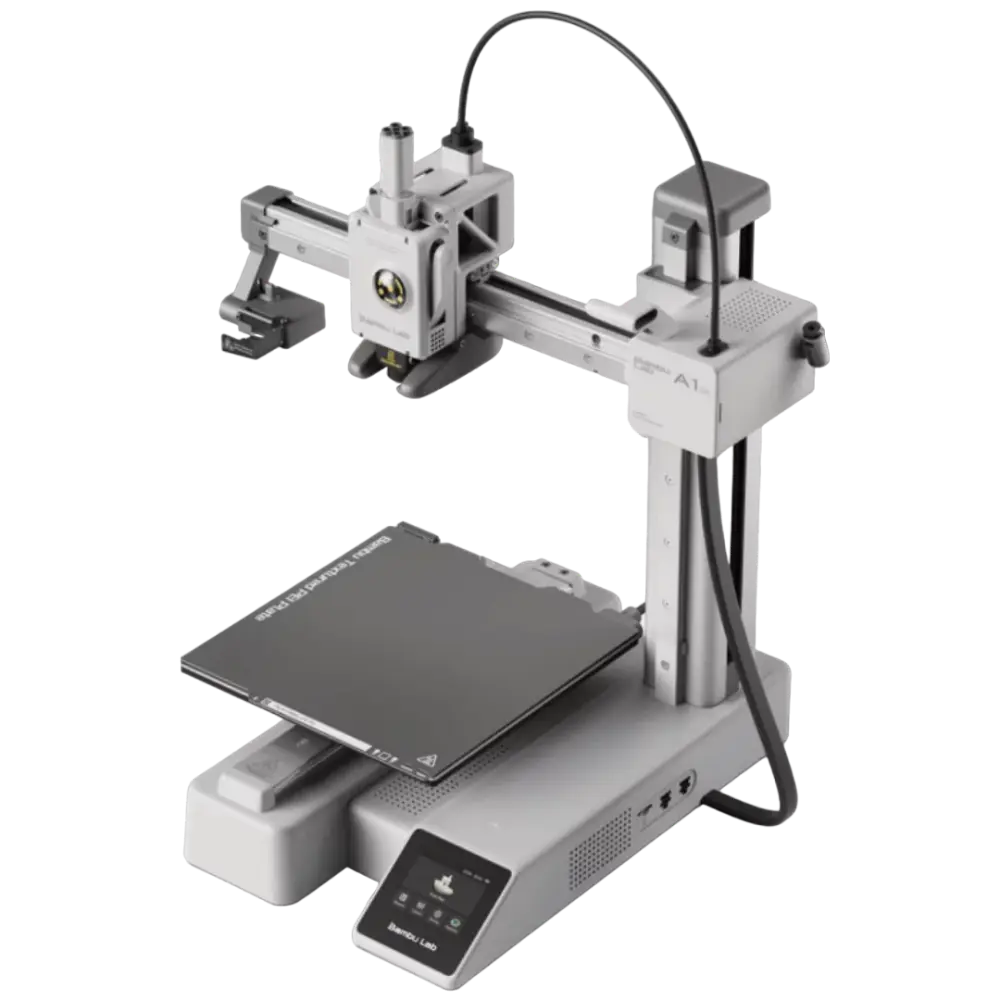
\includegraphics[height=10cm]{a1mini}
  \textbf{\caption{Bambulab A1 mini}}
  \label{fig:a1mini}
\end{figure}

\chapter{Допрограмний етап}
\section{Аналіз об'єкту, що розпізнається}
Необхідно розпізнати робочу поверхню столу FFF 3D принтера Bambulab A1 mini. Дана модель має декілька різних змінних робочих поверхонь, але найбільш розповсюджена -- PEI-пластина.\\
\begin{figure}[h]
  \center
  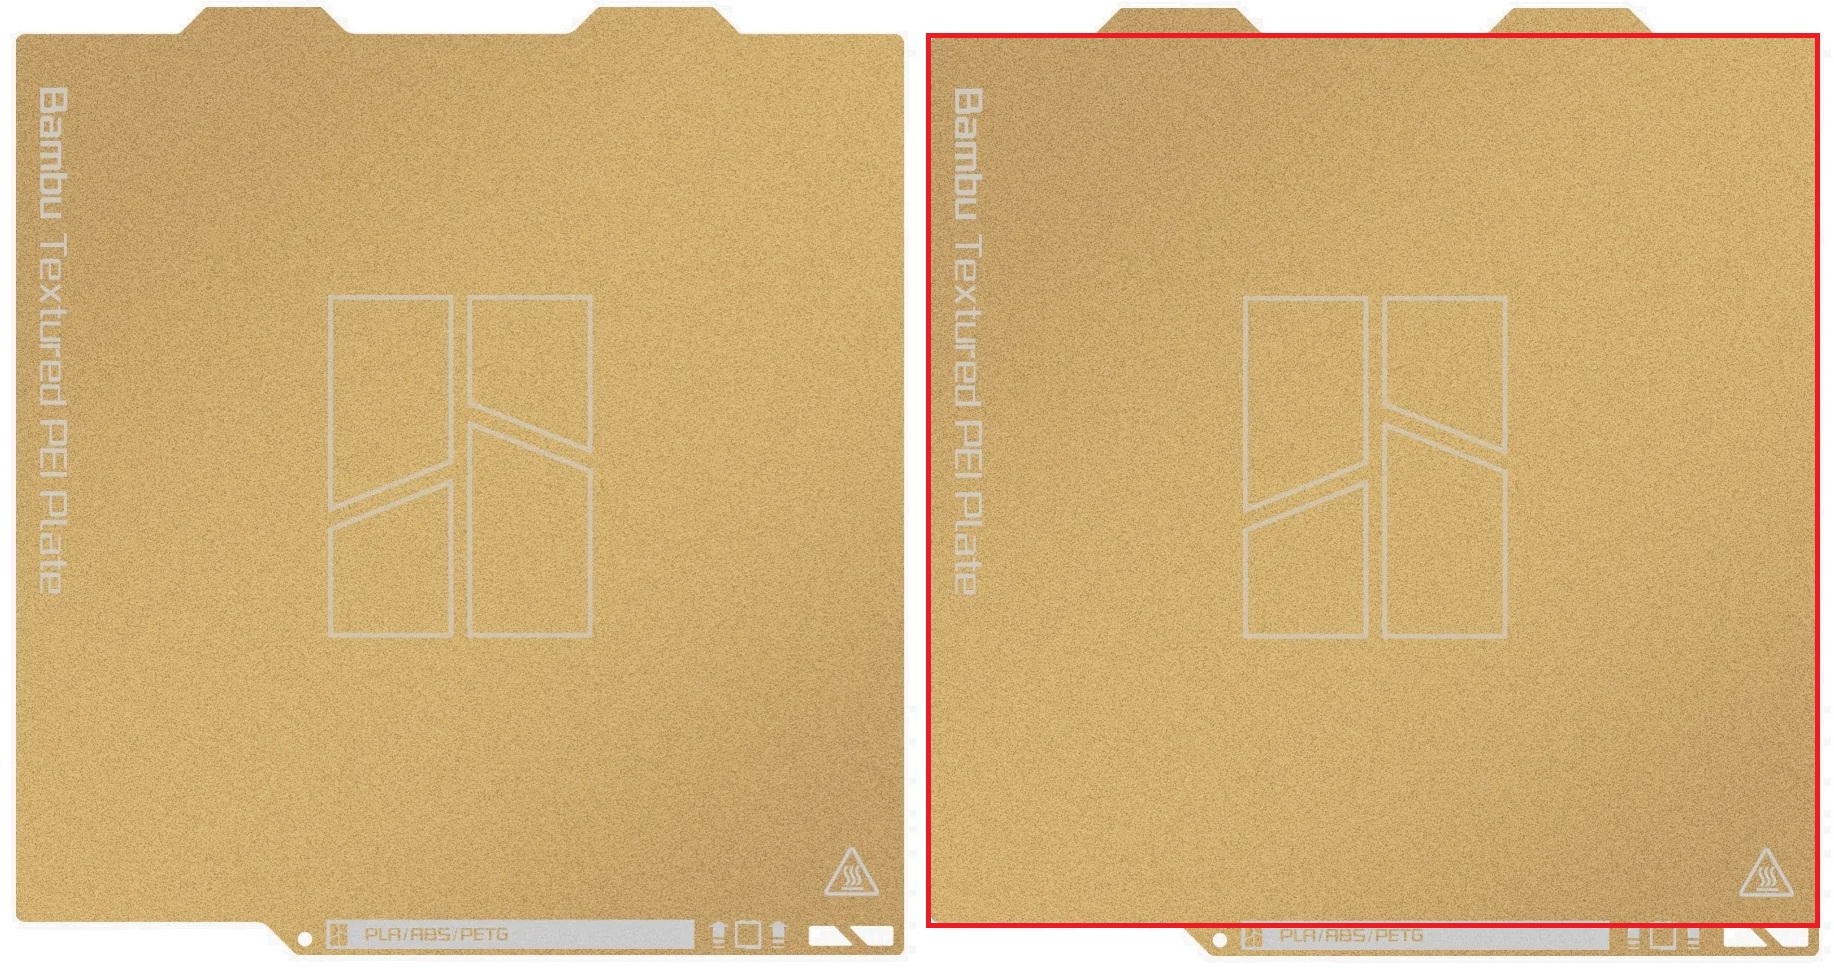
\includegraphics[width=\textwidth]{PEIPlate}
  \textbf{\caption{PEI-пластина, на зображенні справа показано робочу зону}}
  \label{fig:PEI-plate}
\end{figure}

Робоча область PEI-пластини 18х18 см. Колір майже всіх PEI-пластин бронзово-золотистий. Отже, можна спробувати створити методи що шукають на зображенні проєкції квадратів, конкретний колір, або проєкції і колір одночасно.
Також, при використанні кольору як критерію пошуку, можна скористатись тим, що корпус даного 3D принтера в більшості місць білий.\\

Окрім роботи з значеннями пікселів для визначення кольору, можна скористатись тим, що робоча поверхня дуже контрастна з оточенням, корпусом принтера, і застосувати фільтр границь.\\

\section{Створення методів отримання контексту}
\subsection{Отримання контексту з кольору пікселів}
З кольору пікселів можна створити контекст ввівши ідеальне значення кольору і допустимі відхилення. Доцільно це робити використавши HSV (трьохканальна система кольорів "Колірний тон, насиченість, яскравість"), а не RGB (трьохканальна система кольорів "Червоний, зелений, синій"), 
оскільки в HSV можна проігнорувати яскравість та враховувати лише колірний тон і насиченість.\\
Щоб отримати ідеальне значення кольорів столу і корпусу використано фотографію принтеру в типових умовах освітлення, отриману на камеру телефона.\\
\begin{figure}
  \center
  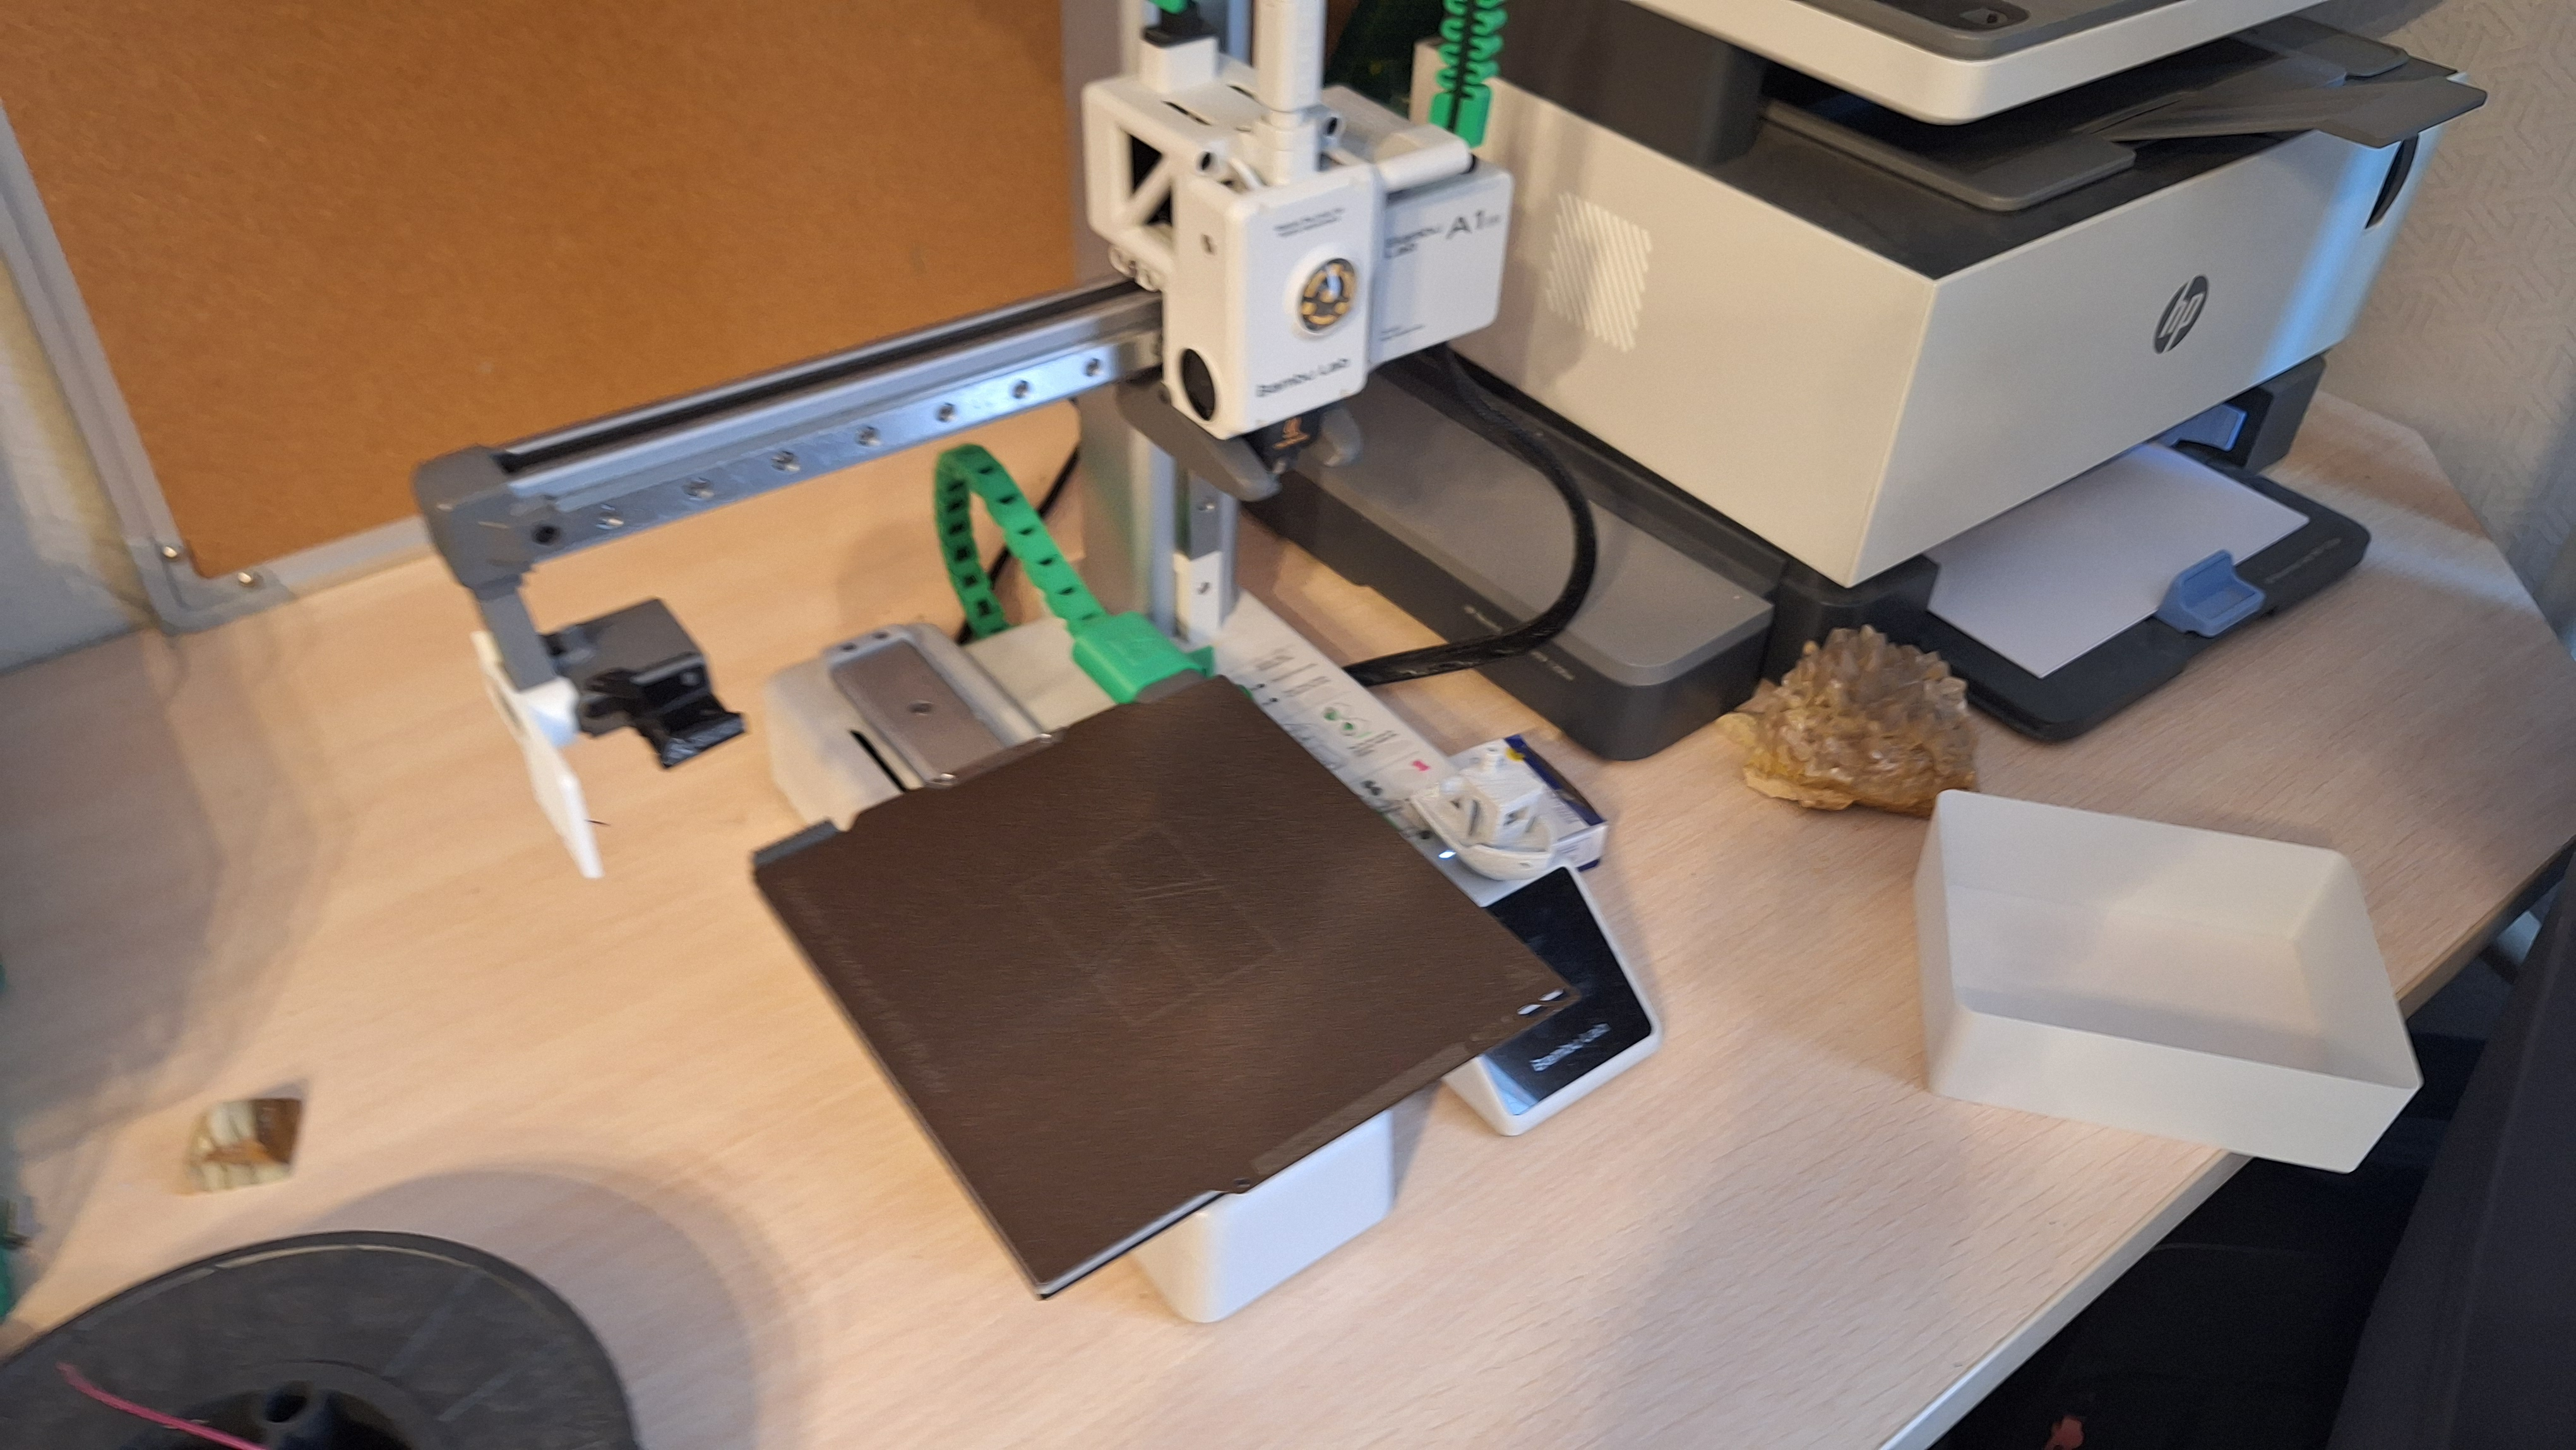
\includegraphics[width=\textwidth]{DSExample1.jpg}
  \textbf{\caption{Зображення принтера отримане за допомогою камери телефона}}
  \label{fig:DSExample1}
\end{figure}

Отримані значення RGB: (89, 65, 55) для столу і (219, 208, 202) для корпусу. Після переходу в HSV отримано (0.05, 0.382, 0.349) і (0.0583, 0.078, 0.859) відповідно. 
Покладено допустимі відхилення тону кольору і насиченості в 0.1 для столу. 
Покладено що насиченість для корпусу має бути менша за 0.2, при будь-якому значенні тону. Дані правила застосовані для даного зображення.\\
\begin{figure}
  \center
  \includegraphics[width=\textwidth]{HSVContext1.png}
  \textbf{\caption{Перший набір правил застосований до зображення: правила для столу червоним, правила для корпусу білим}}
  \label{fig:HSVContext1}
\end{figure}

Застосування даних правил значно зменшило область пошуку столу, проте вона все ще залишається великою. З порівняння верхнього і нижнього зображень видно, що правила для столу спрацьовують для світлих ділянок, а правила для корпусу -- для темних. 
Щоб уникнути таких спрацювань, було додано правило на яскравість: для столу яскравість має бути меншою за середню на зображенні, а для корпусу -- більшою.


\chapter{Висновки}

% Бібліографія
\begin{thebibliography}{9}
\bibitem{euler} Автор1. Назва книги. Видавництво, рік.
\bibitem{article} Автор2. Назва статті // Назва журналу. -- Рік. -- Том. -- С. 100-200.
\end{thebibliography}

\end{document}